\chapter{从微分几何到代数几何}
\section{函数层}
Hausdorff空间 $X$ 的任意点都存在和欧式空间同胚的开集,则构成(拓扑)流形,反过来说流形是由欧式空间粘合起来的 整体结构.在流形上赋予光滑的微分结构则构成光滑的微分流形.微分结构的定义中蕴含了函数可微的要求,这种思想 反应到几何中,即用流形上的函数来研究流形本身,就是我们要谈论的层(sheaf).
\begin{note}[]
给定拓扑空间 $X$ ,符号 $\mathcal{O}_X$ 表示拓扑空间 $X$ 上的环层,即 $X$ 上的一个在环范畴取值的层. $\left(X, \mathcal{O}_X\right)$ 称为拓扑空 间 $X$ 上的赋环空间(ringed space). $\mathcal{O}_X$ 也称为赋环空间上的结构层(structure sheaf).对于拓扑空间上的点 $p \in X$ ,层的茎(stalk)记为 $\mathcal{O}_{X, p}$ .
\end{note}
以上罗列了一些关键概念,在给出详尽的定义和讨论之前,我们先接受一个事实:
微分流形 $X$ 上的可微函数构成可微函数环层 $\mathcal{O}_X$ ,从而微分流形是赋环空间.
微分流形的这一结构,在代数几何中可以类比于概形(scheme).理解层的概念是从微分几何过渡到代数结合的关键思维步骤.

下面讨论如何从微分流形得到层的概念.以陈省身的微分几何为例,为了定义余切空间,需要讨论可微流形 $X$ 上的可微 函数 $f, g \in C^1(X)$ 在固定点 $p \in X$ 附近是否相等.附近是一个需要严格表达的概念,按照分析学的逻辑陈述为: 如 果存在 $p$ 的邻域 $H(p)$ 使得函数限制在邻域上相等,则函数等价,商集为函数芽(germ):
\begin{align*}
\left.f\right|_{H(p)}=\left.g\right|_{H(p)} \Leftrightarrow f \sim g \Leftrightarrow[f]=[g] \in C_p^1(X) / \sim
\end{align*}
这是一个极限过程,在比较两个函数 $f, g \in C^1(X)$ 在固定点 $p \in X$ 附近是否局部相等的过程中,需要缩小 $p$ 的邻 域,直到出现邻域 $H(p)$ 满足 $\left.f\right|_{H(p)}=\left.g\right|_{H(p)}$ .
\subsection{预层}
微分几何研究的是具有微分结构的微分流形,其底层的结构是拓扑空间,即拓扑空间范畴 Top 中的对象 $(X, \tau) \in \mathrm{Ob}(\mathbf{T o p})$ .层是对拓扑空间 $X$ 中开集之间相互关系的范畴化描述,为了方便讨论,以拓扑空间 $(X, \tau)$ 中 的开集为对象:
\begin{align*}
U, V \in \tau
\end{align*}
根据其包含(inclusion)关系规定态射
\begin{align*}
\operatorname{Hom}(V, U)= \begin{cases}\left\{\rho_{U V}\right\}, & V \subseteq U \\ \varnothing, & V \nsubseteq U\end{cases}
\end{align*}
这样构造出的拓扑空间 $X$ 上的开集范畴记为 $\mathfrak{T} \mathfrak{o p}(X)$ ,它描述了拓扑空间中开集之间的包含关系,若集合有包含关系 $V \subseteq U$ 则 $V \hookrightarrow U$ 构成包含映射.
我们希望为拓扑空间的每一个开集赋予一个代数结构,这个结构是一个有零对象(zero object)的范畴 $\mathcal{C}$ 中的对象.此 外,对于拓扑空间中开集的包含关系,也赋予范畴 $\mathcal{C}$ 中对象的态射,构成以下反变函子
\begin{align*}
\mathscr{F}: \mathfrak{T o p}(X)^{\mathrm{op}} \rightarrow \mathcal{C}
\end{align*}
称为拓扑空间 $X$ 上的 $\mathcal{C}$ 预层(presheaf),它赋予拓扑空间的每个空间以一个 $\mathcal{C}$ 中的对象,且把拓扑空间中开集的包含关 系对应到 $\mathcal{C}$ 中的态射. $\mathscr{F}(U) \in \mathrm{Ob}(\mathcal{C})$ 为预层在开集上的截面(section).

可微流形 $X$ 上的可微函数集合 $C^1(X)$ 具有自然的函数环的结构.在开集范畴 $\mathfrak{T} o \mathfrak{p}(X)$ 中,给定开集 $U \in \mathrm{Ob}(\mathfrak{T o p}(X))$ ,可微函数环 $C^1(X)$ 限制在 $U$ 上也构成一个函数环 $C^1(U)$ .对于具有包含关系的开集 $V \subseteq U$ ,可微函数环 $C^1(U)$ 限制到 $V$ 上则构成函数环 $C^1(V)$ ,且限制映射是环同态.于是定义可微函数层:
\begin{align*}
\begin{aligned}
\mathscr{F}: \mathfrak{T o p}(X)^{\mathrm{op}} & \rightarrow \text { CRng } \\
U & \mapsto \mathscr{F}(U)=\mathcal{O}(U) \\
V & \mapsto \mathscr{F}(V)=\mathcal{O}(V) \\
\operatorname{Hom}(V, U) & \rightarrow \operatorname{Hom}(\mathcal{O}(U), \mathcal{O}(V))
\end{aligned}
\end{align*}
函子将集合范畴中的包含关系对应到函数的限制即
\begin{align*}
\begin{aligned}
\mathcal{O}(U) & \rightarrow \mathcal{O}(V) \\
u & \left.\mapsto u\right|_V
\end{aligned}
\end{align*}
这样就构建了可微函数预层 $\mathcal{O}_X$ .由于范畴的灵活性,也可以类似定义限制为可微函数预层、 光滑函数预层、 解析函数预层等等.

\subsection{层}
预层描述了开集的包含关系,进一步要考虑拓扑空间的覆盖和粘合,在预层上发展出层的概念.对于预层 $\mathscr{F}: \mathfrak{T} o \mathfrak{p}(X)^{\mathrm{op}} \rightarrow \mathcal{C}$ ,若对于任意开集上的开覆盖 $\left\{U_k\right\} \supseteq U$ ,以下映射
\begin{align*}
\longrightarrow \mathscr{F}(U) \longrightarrow \prod \mathscr{F}\left(U_i\right) \rightrightarrows \prod \mathscr{F}\left(U_i \cap U_j\right)
\end{align*}
构成\textbf{均衡子正合序列(equalizer exact sequence)},那么就称预层为\textbf{层(sheaf)}.举例说明: 可微流形上的可微函数预层 $\mathcal{O}_X$ 构成可微函数层.对于开集 $U \in \mathrm{Ob}(\mathfrak{T o p}(X))$ ,有开覆盖 $\left\{U_k\right\} \supseteq U$ .通过层函子得到限制在 $U$ 的可微函数 环 $\mathcal{O}(U)$ .

\begin{enumerate}
  \item 对于可微函数 $f \in \mathcal{O}(U)$ ,预层的结构有 $\left.f \mapsto f\right|_{U_i}$ 的限制过程.如果它限制在所有的覆盖上都有 $\left.f\right|_{U_i}=0$ 那么 $f=0$ .也就是说,\textbf{预层函子在覆盖 $\left\{U_k\right\}$ 上的\textit{退化 (vanish) (到零对象)} 要求预层函子在被覆盖的开集 $U$ 退化.}

  \item 以上的均衡子正合序列要求,当预层函子在覆盖 $\left\{U_k\right\}$ 上产生相等关系,即对于 $f_i\bigl| \,\in \mathcal{O}\left(U_i\right)\bigr.$ 和 $f_j\bigl|\,\in \mathcal{O}\left(U_j\right)\bigr.$ 这两个来自不同函数环的函数,\textcolor[rgb]{0.66,0.15,0.39}{ 当 $U_i \cap U_j \neq \varnothing$ 即开集相交时,限制在交集上有 $\left.f_i\right|_{U_i \cap U_j}=\left.f_j\right|_{U_i \cap U_j}$ ,此时要求存在唯一的 $f \in \mathcal{O}(U)$ 使得 $\left.f\right|_{U_i}=f_i$ }.也就是说,\textbf{对于开覆盖中相交的开集,在交集上两边的函数相等,产生了粘合的效果}.
\end{enumerate}

\begin{key}
概括而言,在预层中,通过函子 $\mathscr{F}: \mathfrak{T} \mathfrak{o p}(X)^{\mathrm{op}} \rightarrow \mathcal{C}$ 的作用,开集的包含关系对应到 $\mathcal{C}$ 范畴中代数结构的态射关系,\textbf{在固定点上开邻域 (作为开集) 缩小的极限过程对应了 $\mathcal{C}$ 范畴中代数结构的局部化过程}.
在层中,不仅有这样的局部化过程,而且\textbf{通过覆盖上的均衡子正合的要求,确保在开集的交集 $U_i \cap U_j$ 上,代数结构是相容的},反过来说,整个层也可以视为不同的开集\textbf{粘合(glue)}的结果,而\textbf{粘合的重叠部分要靠这种相容性来保障}.
\end{key}
微分几何提供了绝好的例子.可微流形的定义中所谓的\textbf{坐标卡(chart)}和\textbf{图集(atlas)},其实就是对拓扑空间 $X$ 带有局部坐 标系的开覆盖.坐标卡之间的相容性是定义在有相邻关系的坐标卡/开覆盖之间的,即\textbf{在交集上要求相容,而这种相容性 就体现在层中}.

令 $\mathscr{F}: \mathfrak{T o p}(X) \rightarrow \mathcal{O}_X$ 为可微函数层,取拓扑空间 $X$ 中交集 $U \cap V \neq \varnothing$ 非空的两个开集,其并集 $U \cup V$ 被对 应到 $\mathscr{F}(U \cup V)$ ,考虑任意可微函数限制在交集上
\begin{align*}
\begin{aligned}
\mathscr{F}: \mathfrak{T} \mathfrak{\circ p}(X) & \rightarrow \mathcal{O}_X \\
U & \mapsto \mathscr{F}(U) \\
V & \mapsto \mathscr{F}(V) \\
U \cap V & \mapsto \mathscr{F}(U \cap V)
\end{aligned}
\end{align*}

如果有两个可微函数 $u=\mathscr{F}(U)$ 和 $v=\mathscr{F}(V)$ ,它们限制在交集上相等:
\begin{align*}
\left.u\right|_{U \cap V}=\left.v\right|_{U \cap V} \in \mathscr{F}(U \cap V)
\end{align*}
这样相当于可微函数 $u$ 和 $v$ 在交集上粘合起来了,这种粘合表示为层的操作:
\begin{align*}
\mathscr{F}(U) \times \mathscr{F}(U) \rightarrow \mathscr{F}(U \cap V)
\end{align*}
\subsection{茎}
预层 $\mathscr{F}: \mathfrak{T o p}(X)^{\mathrm{op}} \rightarrow \mathcal{C}$ 为每个开集赋予了 $\mathcal{C}$ 范畴中的代数结构.如果需要进一步局部地考虑拓扑空间上的一点 $p \in X$ 则需要茎的概念.
点 $p \in X$ 的一组开邻域 $\left\{U_k(p)\right\} \subset \mathrm{Ob}(\mathfrak{T} \mathfrak{o p}(X))$ ,其中的每个邻域 $U_k(x)$ 又可以确定 $\mathscr{F}\left(U_k(x)\right)$ ,即
\begin{align*}
p \mapsto\left\{U_k(p)\right\} \mapsto\left\{\mathscr{F}\left(U_k(p)\right)\right\}
\end{align*}
取 $U_k(p)$ ,并随之取 $f \in \mathscr{F}\left(U_k(p)\right)$ ,得到二元组 $\left(U_k(p), f\right)$ .考虑两个拓扑上相交的二元组 $\left(U_1(p), f_1\right)$ 和 $\left(U_2(p), f_2\right)$ ,如果存在开集 $U(p)$ :
\begin{align*}
x \in U(p) \subset U_1(p) \cap U_2(p)
\end{align*}
使得 $f_1$ 和 $f_2$ 限制在这个邻域中的值相等,那么便定义等价关系
\begin{align*}
\left.f_1\right|_{U(p)}=\left.f_2\right|_{U(p)} \Leftrightarrow\left(U_1(p), f_1\right) \sim\left(U_2(p), f_2\right)
\end{align*}
根据这个等价关系,可以构造商集:
\begin{align*}
\mathscr{F}_p=\left\{\left(U_k(p), f\right): f \in \mathscr{F}\left(U_k(p)\right)\right\} / \sim
\end{align*}
称为 $\mF$ 的\textbf{茎(stalk)}.

不难理解,茎体现了预层的局部相等的关系,在微分几何中就是函数芽.前面提到函数芽的构造是一个极限过程,在比 较两个函数 $f, g \in C^1(X)$ 在固定点 $p \in X$ 附近是否局部相等的过程中,需要缩小 $p$ 的邻域,直到出现邻域 $H(p)$ 满足 $\left.f\right|_{H(p)}=\left.g\right|_{H(p)}$ .
用范畴的语言定义这个极限过程更加简洁.以固定点 $p \in X$ 为内点的邻域,构成了范畴 $\mathfrak{T} \mathfrak{o p}(X)$ 中的一组对象 $\left\{U_k\right\}$ .在预层 $\mathscr{F}: \mathfrak{T o p}(X)^{\mathrm{op}} \rightarrow \mathcal{C}$ 的作用下,这组对象对应到 $\left\{\mathscr{F}\left(U_k\right)\right\}$ ,茎就是它们的余极限:
\begin{align*}
\mathscr{F}_p=\lim _{\longrightarrow}\left\{\mathscr{F}\left(U_k\right)\right\}
\end{align*}
对于函数层的情形, $f \in \mathscr{F}(U)$ 在这个余极限中的值就是 $f$ 在 $p$ 点的函数芽.
\section{Appendix: 一些范畴论的概念}
\textbf{极限/余极限[Vakil2017]:}

Then the \textbf{limit of the diagram} is an object ${\lim\limits_{\longleftarrow}}_{\sI} A_i$ of $\mathscr{C}$ along with morphisms
$f_j\colon {\lim\limits_{\longleftarrow}}_{\sI} A_i\to A_j$ for each $j\in \sI$, such that $m\colon j\to k$ is a morphism in $\sI$, then 
\begin{center}
\begin{tabular}{rcl}
  \begin{tikzcd}[>=Stealth]
    {\lim\limits_{\longleftarrow}}_{\sI} A_i \arrow[d,"f_j",swap] \arrow[dr,"f_k"] &\\ 
    A_j \arrow[r,"F(m)",swap]& A_k
  \end{tikzcd}
&  
    \begin{tikzcd}[>=Stealth]
      {\lim\limits_{\longleftarrow}}_{\sI} A_i \arrow[dr,"f_i",swap] & \arrow[l,"g",swap] W   \arrow[d,"g_i",swap] \arrow[dr,"f_k"] &\\
      &A_j \arrow[r,"F(m)",swap] &A_k 
    \end{tikzcd}
&
\begin{tikzcd}[>=Stealth]
    {\lim\limits_{\longrightarrow}}_{\sI}A_i  &\\ 
    A_j  \arrow[u,"f_j"] & A_k \arrow[l,"F(m)"]\arrow[ul,"f_k",swap]
  \end{tikzcd}
\end{tabular}\\
\begin{tabular}{p{.3\linewidth}<{\centering} p{.3\linewidth}<{\centering} p{.3\linewidth}<{\raggedright}}
( Fig 1.) & ( Fig 2.) & \hspace{2.5em}( Fig 3.)
\end{tabular}
  \end{center}
commutes, and this object and maps to each $A_i$ are universal (final) with respect to this property. More precisely, given any other object $W$ along with maps $g_i: W \rightarrow$ $A_i$ commuting with the $F(m)$ (if $m: j \rightarrow k$ is a morphism in $\mathscr{I}$, then $\left.g_k=F(m) \circ g_j\right)$, then there is a unique map
\begin{align*}
g: W \rightarrow {\lim\limits_{\longleftarrow}}_{\sI} A_i
\end{align*}
so that $g_i=f_i \circ g$ for all $i$. (In some cases, the limit is sometimes called the inverse limit or projective limit. We won't use this language.) By the usual universal property argument, if the limit exists, it is unique up to unique isomorphism. See (Fig 2.)

\paragraph{Colimits.} More immediately relevant for us will be the dual (arrowreversed version) of the notion of limit (or inverse limit). We just flip the arrows $f_i$ in (Fig 1.), and get the notion of a \textbf{colimit}, which is denoted ${\lim _{\longrightarrow}}_{\sI} A_i$. (You should draw the corresponding diagram. See (Fig 3.)) Again, if it exists, it is unique up to unique isomorphism. (In some cases, the colimit is sometimes called the \textbf{direct limit}, \textbf{inductive limit}, or \textbf{injective limit}. We won't use this language. I prefer using limit/colimit in analogy with kernel/cokernel and product/coproduct. This is more than analogy, as kernels and products may be interpreted as limits, and similarly with cokernels and coproducts. Also, I remember that kernels ``map to", and cokernels are ``mapped to", which reminds me that a limit maps to all the objects in the big commutative diagram indexed by $\mathscr{I}$; and a colimit has a map from all the objects.)

\textbf{均衡子}: 在下图的 $f, g: A \rightarrow B$ 映射中,极限 $K$ 构成了\textbf{均衡子(equalizer)}.

  \begin{center}
  \begin{tikzcd}[>=Stealth]
    K\arrow[r,"k"] & A \arrow[r,"f", bend left=30] \arrow[r,"g", bend right=30] &B
  \end{tikzcd}
\end{center}

平凡(trivial)的条件,指的是纤维丛可以通过简单的直积 $E=X \times F$ 来做投射 $\pi: E=X \times F \rightarrow X$ ,这样就有了标准纤维 $F$ ,它常常是一个张量,用于构造微分流形 $X$ 上的各种张量丛.
\section{向量丛}
标准纤维为向量空间的情况特别值得讨论,它构成了向量丛的理论.重要原因之一在于线性空间范畴中的自同构,也就 是一般线性群的研究构成了群表示论的基础.在前面流形的回顾中,注意到相交坐标卡之间的坐标函数转换问题,概括而论:
\begin{description}
    \item[开覆盖之交集]:拓扑中的粘合等价
    \item[坐标卡之交集]:微分流形中的相容结构
    \item[开覆盖的截面之转换]:向量丛的G-群
\end{description}

丛拓扑商空间,到微分流形坐标卡,到向量丛的G-群,是逐步添加数学结构的过程.
丛的构造视为不交并.若邻近的开集相交处有两点 $(p, v) \in U_i \times V$ 和 $\left(p, v^{\prime}\right) \in U_j \times V$ ,虽然根据拓扑的粘合映射 它们在底空间是同一点,但需要考虑标准纤维上两个向量的等价关系 $v \sim v^{\prime}$ .考虑 $V$ 上的变换群 $G$ ,由于可逆和线 性的要求通常要求 $G$ 是一般线性群 $G=\operatorname{GL}(n, K)$ 或者其子Lie群,即用某种可逆线性变换群将 $v$ 和 $v^{\prime}$ 联系起来. 对于邻近的开集可以在交集上定义\textbf{转移函数(transition function)}
\begin{align*}
\begin{aligned}
g_{i j}: U_i \cap U_j & \rightarrow G \\
p & \mapsto g_{i j}(p)
\end{aligned}
\end{align*}
它是标准纤维上的线性自态射:
\begin{align*}
\begin{aligned}
g_{i j}(p): V & \rightarrow V \\
v & \mapsto\left(g_{i j}(p)\right)(v)
\end{aligned}
\end{align*}
当满足 $v=g_{i j} v^{\prime}=\left(g_{i j}(p)\right)\left(v^{\prime}\right)$ 时,建立了 $v \sim v^{\prime}$ 的关系,这两点相当于等同.等价关系要求变换群的可逆,于是自然地让变换群放置在一般线性群或者Lie群的框架下研究,这样构造的向量丛为\textbf{G-丛(G-bundle)}.在规范理论中,一个标准纤维 $V$ 和作用其上的规范变换群 $G$ ,可以在流形 $M$ 上相应构造G-丛,而场就是 $G$-丛上的截面(section).

向量丛的构建还要求以上的条件,使得指标的循环构成了复合变换群退化为恒同,这个条件称为\textbf{上闭链(cocycle)条件}.\textbf{它暗示覆盖的交集部分蕴含着拓扑信息,可以通过有序指标的代数方法来讨论};而上闭链强烈提示我们这里打开了通向上同调理论的大门.

\section{多项式环素谱上的Zariski拓扑}
代数几何研究多项式的解集, 在代数封闭域 $K$上, $n$--维仿射空间 $K^n$ 有$K$--多项式环
\[K[x]=K[x_1,x_2,\cdots,x_n],\]
它是 $K^n\to K$多项式的全体, 并由 $K$上的运算赋予自然的环的加法、乘法和相应幺元. \textbf{图\ref{fig: zariski maps}} 给出了常见的映射关系. 带框的部分表示可以定义Zariski拓扑, 图中体现了文中 \eqref{eq:zero set4} \eqref{eq:zero set8}这两个Zariski拓扑和 \eqref{eq:zero set6} Hilbert零点定理:
\begin{figure}[h]
  \centering
\begin{tikzpicture}[]
  \node[] (11) at (0,0) {$K$};
  \node[below,yshift=-2cm] (21) at (11.south) {\fbox{$K^n$}};
  \node[right,xshift=3cm] (22) at (21.west) {$K[x]$};
  \node[right,xshift=2.5cm] (23) at (22.west) {$\textrm{Ideal}(K[x])$};
  \node[right,xshift=5cm] (24) at (23.west) {\fbox{$\textrm{Spec}(K[x])$}};
  \node[below,yshift=-4cm] (41) at (21.south) {\fbox{$Z(S)=Z(\mathfrak{s})$}};
  \node[below,yshift=-1.5cm] (32) at (22.south) {$S$};
  \node[below,yshift=-1.45cm] (33) at (23.south) {$\mathfrak{s}=(S)$};
  \node[below,yshift=-4.2cm] (43) at (23.south) {$I(Z(\mathfrak{s}))=\sqrt{\mathfrak{s}}$};
  \node[below,yshift=-3.9cm] (44) at (24.south) {\fbox{$V_I=\{\mathfrak{a}\in \operatorname{Spec}(K[x])\mid \mathfrak{a}\supset I\}$}};
  \draw[->] (21) --node[left] {$f\in K[x]$} (11);
  \draw[->,dashed] (41) --node[left] {\rotatebox{90}{$\subset$}} (21);
  \draw[dashed] (21) -- (22);
  \draw[dashed] (22) --node[above] {$\subset$} (23);
  \draw[dashed] (23) --node[above] {$\subset$} (24);
  \draw[->,dashed] (32) --node[left] {\rotatebox{90}{$\subset$}} (22);
  \draw[->] (33) --node[left] {\rotatebox{90}{$\in$}} (23);
  \draw[->] (32) --node[left] {$Z$} (41);
  \draw[->] (33) --node[right,shift={(0,5pt)}] {$V$} (44);
  \draw[->] (33) --node[right,yshift=-5pt] {$Z$} (41);
  \draw[->] (41) --node[below] {$I$} (43);
  \draw[->] (33) --node[left] {$I\circ Z$} (43);
  \draw[->] (44) --node[left] {\rotatebox{90}{$\subset$}} (24);
  \draw[->] (32) --node[above] {$\textrm{Ideal}$} (33);
\end{tikzpicture}
  \caption{Zariski拓扑常见映射关系}
  \label{fig: zariski maps}
\end{figure}

孤立点、紧的圆周、嵌入在高维空间的直线、超平面、曲面... 这些都可以构成多项式集合的解集,从直观上人们感觉这些解集是闭集,相应地解集的补集是开集.这种直观通过Zariski拓扑的方式严格表述为Zariski拓扑,后面我们将讨论几个不同的Zariski拓扑空间的关系.
\clearpage
\subsection{理想}
\textbf{在环论中理想的地位 (构造商环) 相当于群论中的正规子群 (构造商群)} . 我们注意到对理想的研究远远地多于子环, 这是因为理想是一类特殊的子环:
\begin{figure}[htbp]
  \small
  \centering
  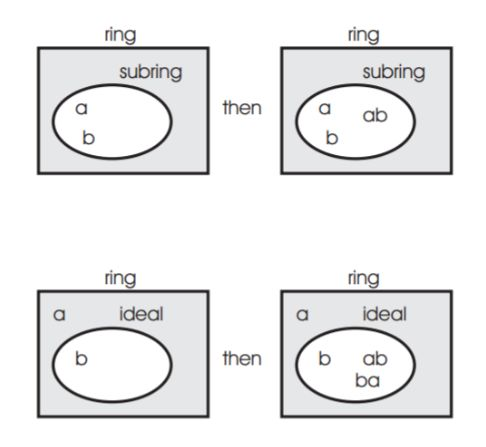
\includegraphics[width=.5\linewidth]{subrings and ideals}
  \caption{子环与理想的对比}
  \label{fig: the difference between subring and ideal}
\end{figure}

\textbf{对于环 $R$ 理想 $I$ ,不仅要求理想自身作为子环的环乘封闭,还要求理想对 $R \backslash I$ 中环元能够环乘封闭,故理想 $I$ 比子环 更多反映出环 $R$ 本身的性质,而子环 $R^{\prime}$ 已经可以完全无视 $R \backslash R^{\prime}$ 的影响.}
理想的加法和乘法定义如下:
\begin{align*}
\mathfrak{a}+\mathfrak{b}=\{a+b \mid a \in \mathfrak{a} \text { and } b \in \mathfrak{b}\}
\end{align*}
以及
\begin{align*}
\mathfrak{a} \mathfrak{b}=\left\{\sum_{k=1}^n a_k b_k \mid a_k \in \mathfrak{a}, b_k \in \mathfrak{b}\right\}
\end{align*}
环 $R$ 中的子集 $S \subset R$ 生成的理想记为 $(S)$ .

\subsection{多项式环}

以下映射给出了多项式的公共零点集
\begin{equation}\label{eq:zero set1}
\begin{aligned}
Z: 2^{K[x]} & \rightarrow K^n \\
S & \mapsto Z(S)=\left\{x \in K^n \mid \forall f \in S: f(x)=0\right\}
\end{aligned}
\end{equation}
,这里的 $2^{K[x]}$实则为 $K[x]$的幂集.
$K^n$ 中的子集,如果可以表示为多项式集合的公共零点集,称为代数集(algebraic set). \cite{hartshorne2013algebraic}  给出了代数 集上的Zariski拓扑(Zariski topology),相应地将 $K^n$ 上的闭集构成的集族记为 $\overline{\mathfrak{T} o p}\left(K^n\right.$ ) (这里借用了开集范畴的记号) .

\begin{proposition}
  The union of two algebraic sets is an algebraic set. The intersection of any family of algebraic sets is an algebraic set. The empty set and the whole space are algebraic sets.
\end{proposition}
\begin{proof}
  If $Y_1=Z\left(T_1\right)$ and $Y_2=Z\left(T_2\right)$, then $Y_1 \cup Y_2=Z\left(T_1 T_2\right)$, where $T_1 T_2$ denotes the set of all products of an element of $T_1$ by an element of $T_2$. Indeed, if $P \in Y_1 \cup Y_2$, then either $P \in Y_1$ or $P \in Y_2$, so $P$ is a zero of every polynomial in $T_1 T_2$. Conversely, if $P \in Z\left(T_1 T_2\right)$, and $P \notin Y_1$ say, then there is an $f \in T_1$ such that $f(P) \neq 0$. Now for any $g \in T_2,(f g)(P)=0$ implies that $g(P)=0$, so that $P \in Y_2$.

If $Y_x=Z\left(T_x\right)$ is any family of algebraic sets, then $\bigcap Y_x=Z\left(\bigcup T_\alpha\right)$, so $\bigcap Y_\alpha$ is also an algebraic set. Finally, the empty set $\varnothing=Z(1)$, and the whole space $\mathbf{A}^n=Z(0)$.
\end{proof}
\begin{definition}
  We define the Zariski topology on $\mathbf{A}^n$ by taking the open subsets to be the complements of the algebraic sets. This is a topology, because according to the proposition, the intersection of two open sets is open, and the union of any family of open sets is open. Furthermore, the empty set and the whole space are both open.
\end{definition}

反过来考虑:
\begin{equation}\label{eq:zero set2}
\begin{aligned}
I: K^n & \rightarrow 2^{K[x]} \\
Y & \mapsto I(Y) \\
& =\{f \in K[x] \mid \forall x \in Y: f(x)=0\} \\
& =\{f \in K[x] \mid Y \subset Z\{f\}\}
\end{aligned}
\end{equation}
即 $I(Y)$ 是解集包含 $Y$ 的多项式的集合.

多项式环上定义的乘法和多项式的理想有密切的关系,若 $Y=Z(S) \subset K^n$ 是一组多项式 $S \in K^n$ 的解集,显然 $I(Y)$ 是 $K^n$ 的子环,多项式的乘法确保了 $\forall f \in I(Y)$ 和任意环元 $p \in K^n$ 的乘积 $f p$ 的解集仍然包含 $Y$ ,于是 $I(Y)$ 构成一个理想.为了研究代数集 $Y$ ,往往要考虑限制在 $Y$ 上相等的多项式等价类 (类似函数芽在邻域相等), $Y$ 确定的这个理想诱导了一个商环,称为 $Y$ 的坐标环(coordinate ring)或者结构环(structure ring):
\begin{align*}
K[x] / I(V)
\end{align*}
任意取 $g \in K[x]$ 有
\begin{align*}
\forall f \in S, x \in Y:(f g)(x)=f(x) g(x)=0 \Rightarrow x \in Z(f g)
\end{align*}
它满足了理想中对任意环元的封闭性,于是可以考虑由 $S$ 生成的理想
\begin{align*}
\mathfrak{s}=(S) \in \operatorname{Ideal}(K[x])
\end{align*}
对于任意 $x \in Y$ 和 $f \in S$ 都满足 $f(x)=0$ ,故 $x$ 也是它生成的理想中的零点,即 $Z(S) \subseteq Z(\mathfrak{s})$ .又由于 $S \subseteq \mathfrak{s}=(S) \subseteq K^n$ ,有 $Z(S) \supseteq Z(\mathfrak{s})$ .于是
\begin{equation}\label{eq:zero set3}
Z(S)=Z(\mathfrak{s})
\end{equation}
由于交换代数的成果,后面的讨论将从多项式环 $K[x]$ 转向环上的理想的集合 $\operatorname{Ideal}(K[x])$ .由于多项式集的零点集 可以直接替换为多项式集生成的理想的零点集,于是有了对应:
\begin{equation}\label{eq:zero set4}
\begin{aligned}
Z: \operatorname{Ideal}(K[x]) & \rightarrow \overline{\mathfrak{T} \mathfrak{o p}}\left(K^n\right) \\
\mathfrak{s} & \mapsto Z(\mathfrak{s})
\end{aligned}
\end{equation}
\subsection{Hilbert零点定理}
\eqref{eq:zero set4}和\eqref{eq:zero set2}的复合映射为
\begin{equation}\label{eq:zero set5}
  \begin{aligned}
  I \circ Z: \operatorname{Ideal}(K[x]) & \rightarrow \operatorname{Ideal}(K[x]) \\
  \mathfrak{s} & \mapsto I(Z(\mathfrak{s}))
  \end{aligned}
  \end{equation}
  构成了 $K[x]$ 的理想到理想的映射.\textbf{Hilbert零点定理 (Hilbert's Nullstellensatz)} 给出了重要的对应:
  \begin{equation}\label{eq:zero set6}
  \mathfrak{s} \subset I(Z(\mathfrak{s}))=\sqrt{\mathfrak{s}}=\left\{r \in K[x] \mid \exists n \in \mathbb{Z}^{+}: r^n \in \mathfrak{s}\right\}
  \end{equation}
  这样 $K^n$ 中的代数集、 $K[x]$ 中多项式的理想、根理想都对应起来了.
  在拓扑空间中,非空子集若不能表示为两个非空闭真子集的并,则称为\textbf{不可约的 (irreducible)}.在Zariski拓扑下, 不可约 的代数集称为代数簇(algebraic variety).\cite{hartshorne2013algebraic}

  \begin{theorem}[][Hilbert's Nullstellensatz]
    Let $k$ be an algebraically closed field. Let $\mathfrak{a}$ be an ideal in $A=k[x_1,\cdots,x_n]$ and let $f\in A$ be an polynomial which vanishes at all poits of $Z(\mathfrak{a})$. Then $f^r\in \mathfrak{a}$ for some integer $r>0$.
  \end{theorem}
\begin{proof}
  Lang [1,p.256]\cite{lang2012algebra} or Atiyah-Macdonald [1,p.285] or Zariski-Samual [1,vol. 2., p. 164].
\end{proof}
\begin{corollary}
  There is a one-to-one inclusion-reversing correspondence between algebraic sets in $A^n$  and radical ideals (i.e. ideals which equal to their own radical) in $A$, given by $Y\mapsto I(Y)$ and $\mathfrak{a}\mapsto Z(\mathfrak{a})$. Furthermore, an algebraic set is irreducible if and only if its ideal is a prime ideal.
\end{corollary}

Hilbert零点定理给出了代数集 $Y$ 和根理想 $\sqrt{Y}$ 的对应,而代数集能够构成代数簇的不可约的条件则对应着素理想 (prime ideal),即要求 $I(Y)$ 是素理想,这一条件也相当于 $Y$ 的坐标环 $K[x] / I(Y)$ 是整环.代数几何研究代数簇, 故后面将集中于对多项式环 $K[x]$ 中素理想的研究.
\subsection{素谱}
环 $R$ 的素理想构成的集合,称为素谱(spectrum),记为 $\operatorname{Spec} R$ .我们将要分三个阶段来理解它:
\begin{enumerate}
  \item 作为集合: 素谱 $\operatorname{Spec} (K[x])$ 是环 $K[x]$ 的素理想构成的集合
  \item 作为拓扑空间
  \item 作为结构层
\end{enumerate}
完成这几个阶段后就得到了仿射概形,也就是概形的局部模型.先考虑素谱上的拓扑.对于任意的理想 $\mathfrak{s} \in \operatorname{Ideal}(K[x])$ ,包含它的素理想的集合记为:
\begin{equation}\label{eq:zero set7}
\begin{aligned}
V: \operatorname{Ideal}(K[x]) & \rightarrow \operatorname{Spec} K[x] \\
\mathfrak{s} & \mapsto V(\mathfrak{s})=\{\mathfrak{a} \in \operatorname{Spec} K[x] \mid \mathfrak{a} \supset \mathfrak{s}\}
\end{aligned}
\end{equation}
其补集记为 $\bar{V}(\mathfrak{s})=\operatorname{Spec} K[x] \backslash V(\mathfrak{s})$ ,
[Atiyah1969] 给出了\textbf{素谱上的Zariski拓扑}:
\begin{definition}[][The prime spectrum of a ring]
  Let $A$ be a ring and let $X$ be the set of all prime ideals of $A$. For each subset $E$ of $A$, let $V(E)$ denote the set of all prime ideals of $A$ which contain $E$. Prove that
\begin{enumerate}[label=\roman*),font=\upshape,leftmargin=1.8em,nosep]
  \item if $\mathfrak{a}$ is the ideal generated by $E$, then $V(E)=V(\mathfrak{a})=V(r(\mathfrak{a}))$.
  \item $V(0)=X, V(1)=\varnothing$.
  \item if $\left(E_i\right)_{i \in l}$ is any family of subsets of $A$, then
  \begin{align*}
  V\Bigl(\bigcup_{i \in I} E_i\Bigr)=\bigcap_{i \in l} V\left(E_i\right) .
  \end{align*}
  \item $V(\mathfrak{a} \cap \mathfrak{b})=V(\mathfrak{a} \mathfrak{b})=V(\mathfrak{a}) \cup V(\mathfrak{b})$ for any ideals $\mathfrak{a}, \mathfrak{b}$ of $A$.
\end{enumerate}

These results show that the sets $V(E)$ satisfy the axioms for closed sets in a topological space. The resulting topology is called the \textbf{Zariski topology}. The topological space $X$ is called \textbf{the prime spectrum of $A$}, and is written $\operatorname{Spec}(A)$.
\end{definition}

类似\eqref{eq:zero set4}, 素谱上的Zariski拓扑的诱导可以写作
\begin{equation}\label{eq:zero set8}
\begin{aligned}
V: \operatorname{Ideal}(K[x]) & \rightarrow \overline{\mathfrak{T} o p}(\operatorname{Spec} K[x]) \\
\mathfrak{s} & \mapsto V(\mathfrak{s})
\end{aligned}
\end{equation}
\eqref{eq:zero set4}和\eqref{eq:zero set8}告诉我们,多项式环 $K[x]$ 中的理想 $\mathfrak{s}$ ,对应着 $K^n$ 上的闭集 $Z(\mathfrak{s})$ 和素谱 $\operatorname{Spec} K[x]$ 上的闭集 $V(\mathfrak{s})$ ,这 样就让素谱上的拓扑的几何意义可以明确地通过 $K^n$ 上的拓扑体现出来.
\clearpage
\section{函数环}
\subsection{函数环的子环}
集合范畴 $\operatorname{Top}$ 中的态射 $f \in \operatorname{Hom}(X, Y)$ ,若关注于(交换) 域 $k$ 则构成 $k$ 值函数.域 $k$ 的交换性赋予 $h_k X$ 逐 点定义的交换环的结构,即函数环,记:
\begin{align*}
f \in C(X)=h_k X=\operatorname{Hom}(X, k) \in \mathbf{C R n g}
\end{align*}
拓扑学讨论的是拓扑空间中的对象 $X \in \mathbf{T o p}$ 上的连续函数环 $C^0(X)$ .微分几何讨论的是可微流形上的可微函数环 $C^1(X)$ 或光滑函数环 $C^{\infty}(X)$ .尽管如此,仍然不方便讨论因式分解的问题,而多项式环 $k[x]$ 则十分方便讨论这些 代数问题,故有讨论范围的逐步精细化:
\begin{equation}\label{eq: function ring1}
k[x] \subset C^{\infty}(X) \subset \cdots \subset C^1(X) \subset C^0(X) \subset C(X)=h_k X
\end{equation}
以上出现的各项都是交换环,可见函数环在交换代数的地位.虽然以上给出了嵌套的子环序列,但环和子环之间缺少联 系.譬如可微函数 $f \in C^1(X)$ 和连续函数 $g \in C^0(X)$ 之间的乘法 $f g$ 并非可以保证可微,作为子环的 $C^1(X)$ 缺少 和 $C^0(X)$ 的有力联系.
\subsection{理想}
在交换代数中,理想远比子环重要,函数环可以自然的发展出理想的概念.令 $R \in \mathbf{C R n g}$ 为\eqref{eq: function ring1}中任何一种函数环, 以下插图来自 $B$ 站 [概形的灵感].以 $X=\mathbb{R}$ 为例随意取了一些函数:
\begin{figure}[htbp]
  \centering
  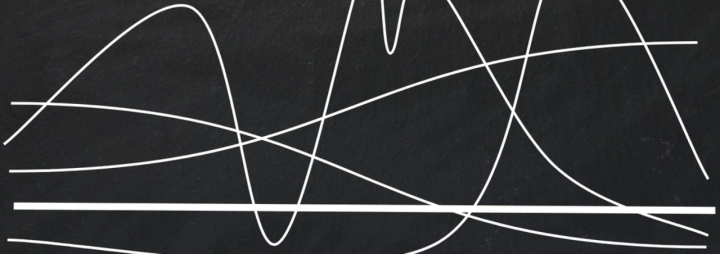
\includegraphics[width=.5\linewidth]{3}
  \caption{函数环上的函数}
  \label{fig: function ring1}
\end{figure}
在函数乘法 $(R,\cdot,1)$下构成交换幺半群(monoid). 这个monoid不能保证乘法逆元存在的根源之一在于存在零点:
\begin{figure}[htbp]
  \centering
  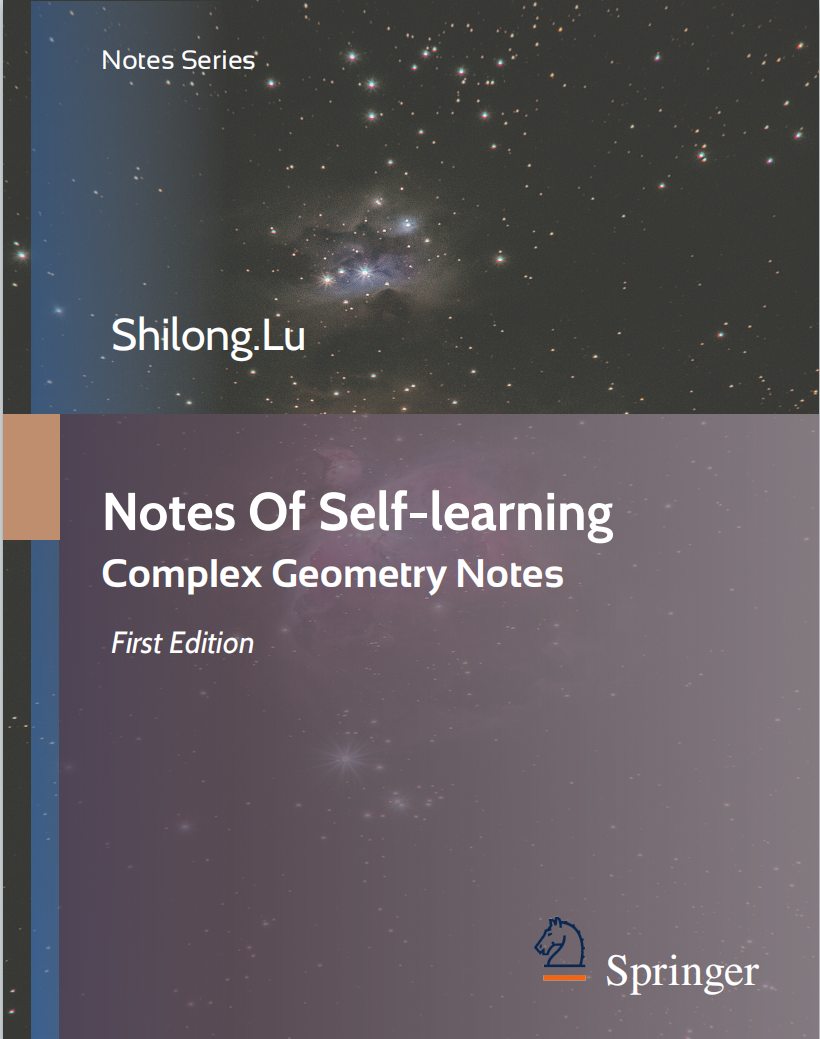
\includegraphics[width=.5\linewidth]{1}
  \caption{函数环上的函数局部图}
  \label{fig: function ring2}
\end{figure}
给定零点 $a\in X$, 解集包含它的函数集记为:
\begin{equation}\label{eq: function ring2}
  I(a)=\{f \in R \mid f(a)=0\}
  \end{equation}
  显然它在函数加法下构成Abel群,并且对于 $\forall f \in R$ 以乘法作用于 $I(a)$ 中的函数,得到的函数仍然以 $a$ 为零点,于是 $f \cdot I(a)=I(a) \cdot f \subseteq I(a)$ ,即 $I(a) \in \operatorname{Ideal} R$ 为函数环中的理想,它通过函数乘法吸收了环 $R$ 中的成员.从商 环 $R / I$ 上看,两个函数 $f_1, f_2 \in R$ 在 $a$ 处相等即有
  \begin{equation*}
  \left(f_1-f_2\right)(a)=0 \Leftrightarrow f_1 \sim f_2 \Leftrightarrow f_1+I=f_2+I
  \end{equation*}
  在多项式环中这种构造就是坐标环,它把函数限定在一个集合上的相等归纳为等价.
  \subsection{素理想}
  考虑两个函数 $f, g \in R$ 在零点上的性质,若 $f \cdot g \in I(a)$ 即 $f(a) \cdot g(a)=0$ ,那么必有 $f(a)=0$ 或者 $g(a)=0$ .于是\eqref{eq: function ring2}中定义的理想是素理想,从点到素理想的诱导过程为:
  \begin{equation}\label{eq: function ring3}
  \begin{aligned}
  X & \rightarrow \operatorname{Spec} R \\
  a & \mapsto I(a)=\{f \in R \mid f(a)=0\}
  \end{aligned}
  \end{equation}
  于是 $X$ 上的点被赋予了素理想的结构.
  对于多于一个零点的情况,譬如 $a, b \in X$ 类似可以考虑
  \begin{align*}
  I(a, b)=\{f \in R \mid f(a)=0, f(b)=0\}
  \end{align*}
  这个集合仍然构成理想.若有两个函数 $f, g \in R$ 使得:
  \begin{itemize}
    \item $f(a)=0, f(b) \neq 0$ 于是 $f \notin I(a, b)$,
    \item $g(a) \neq 0, g(b)=0$ 于是 $g \notin I(a, b)$.
  \end{itemize}
  那么 $(f g)(a)=(f g)(b)=0$ 即 $f g \in I(a, b)$ ,于是 $I(a, b)$ 不是素理想.这就说明了仿射空间上的单个点和素理想的联系的意义所在.

\subsection{局部环}
将上述讨论限制在可微流形$X$上, 构造可微函数环层 $\mO_X$ [MP129]. 在点$p\in X$上则是函数芽的茎$\mO_p$. 对于有零点的函数$f\in \mO_X$, 限制在开集$U\in \mathfrak{Top}(X)$的 $f|_U \in \mO_U$ 可能是没有零点的. 通过限制让有多个零点的函数限制在开集上只有一个零点, 构成素理想. 拓扑空间中的包含关系, 通过层构成环的局部化 (localization).
\begin{figure}[htbp]
  \centering
  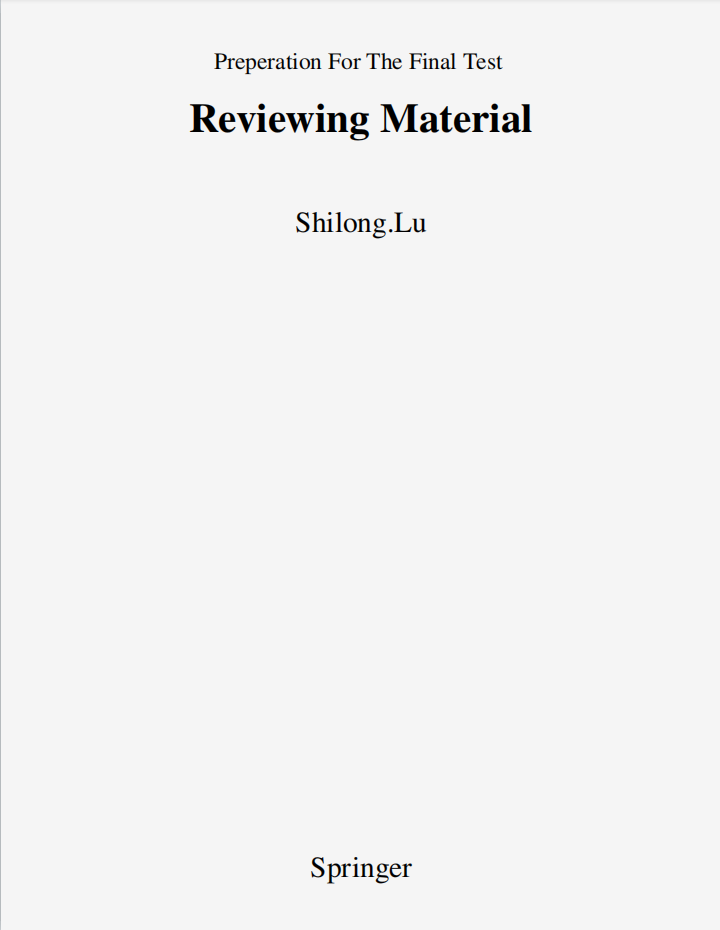
\includegraphics[width=.5\linewidth]{2}
  \caption{函数环的局部化}
  \label{fig: function ring 3}
\end{figure}
在 $p$ 点退化的函数芽的集合记为 $\mathfrak{m}_p$ ,显然它是一个理想,而且它是一个极大理想,只有一个极大素理想的环叫做局部 环(local ring),于是 $\mathcal{O}_p$ 是局部环.
函数芽是函数的局部化,作为一个交换环 $\mathcal{O}_p \in \mathbf{C R n g}$ ,它在环乘法下构成monoid,如前述这个monoid不能保证乘 法逆元存在的原因之一在于存在零点,然而通常而言即使不存在零点,也不能保证函数可逆.
和前面的讨论不同,现在函数芽已经被局部化,且对于可微函数而言局部化意味着线性化一一微分学的基本思想.因 此,函数芽 $f \in \mathcal{O}_p$ 可逆 iff. $f(p) \neq 0$ ,这样有了逆 $1 / f(x)$ .进一步在 $p$ 点非退化的函数芽的集合 $\mathcal{O}_p \backslash \mathfrak{m}_p$ ,在函 数环的乘法下封闭,于是我们构造了一个交换的局部环,且 $\mathfrak{m}_p$ 是 $\mathcal{O}_p$ 中唯一的极大理想.
在实数取值的茎有满态射 $\pi: \mathcal{O}_p \rightarrow \mathbb{R}$ ,且极大理想 $\mathfrak{m}_p \rightarrow \mathcal{O}_p$ 是嵌入,故有短正合序列:
\begin{align*}
0 \longrightarrow \mathfrak{m}_p \longrightarrow \mathcal{O}_p \stackrel{\pi}{\longrightarrow} \mathbb{R} \longrightarrow 0
\end{align*}
于是有同构:
\begin{align*}
\mathcal{O}_p / \mathfrak{m}_p \simeq \mathbb{R}
\end{align*}
构成了剩余域(residue field).这里的关键是自然投射 $\pi$ ,它把具有相同余切向量的函数芽等价到一个等价类中.我们可 以把函数在固定点 $p$ 的取值理解为环对极大理想 $\mathfrak{m}_p$ 的模,这是流形和概形共同的代数基础—一局部赋环空间(locally ringed space).

\section{Hilbert零点定理}
\subsection{退化集}
多项式环的子集 $S \subset k[x]$ 为多项式集,其生成的理想记为 $J=(S)$ ,二者具有相同的代数集
\begin{equation}\label{eq: hilbert zero thm 1}
Z(J)=\left\{a \in A_k^n \mid \forall f \in J \Rightarrow f(a)=0\right\}=Z(S)
\end{equation}
方便起见后面用理想 $J$ 代替集合 $S$ .仿射空间的点 $a \in A_k^n$ 对应着素谱中的点 (素理想) :
\begin{equation}\label{eq: hilbert zero thm 2}
\mathfrak{p}_a=I(a)=\{f \in k[x] \mid f(a)=0\} \in \operatorname{Spec} k[x]
\end{equation}
素理想 $\mathfrak{p}_a$ 由在 $a$ 退化的多项式构成,考虑多项式 $f \in k[x]$ 到商环 $k[x] / \mathfrak{p}_a$ 的投射:
\begin{align*}
f \mapsto f+\mathfrak{p}_a
\end{align*}
环元 $f$ 在 $a$ 退化相当于它处于素理想中 $f \in \mathfrak{p}_a \in \operatorname{Spec} k[x]$ ,则 $f+\mathfrak{p}_a=0$ .于是 $f$ 也可以视为在素谱上的函 数, $f(a)=0$ 在仿射空间的点 $a \in A_k^n$ 上退化,也可视为 $f$ 在 $\mathfrak{p}_a$ 退化 $f\left(\mathfrak{p}_a\right)=0$ .
通过上述操作,定义在仿射空间 $A_k^n$ 中的多项式转变为定义在素谱 $\operatorname{Spec} k[x]$ 上的函数.多项式生成的理想 $J$ 确定了 仿射空间的退化集 $Z(J)$ 即代数集(1),现在则转为讨论素谱上的\textbf{退化集(vanishing set)}:
\begin{equation}\label{eq:hilbert zero thm 3}
V(J)=\{\mathfrak{p} \in \operatorname{Spec} k[x] \mid \forall f \in J \Rightarrow f(\mathfrak{p})=0\}
\end{equation}
这种思想适用于一般的交换环,环元 $f$ 包含于素理想 $\mathfrak{p}$ 相当于环元作为方程在素谱上退化 $f(\mathfrak{p})$ $=0$ . 

\begin{example}[][from [Vakil2017] 3.2.1]
  The set $S p e c A$ is the set of prime ideals of $A$. The prime ideal $\mathfrak{p}$ of $A$ when considered as an element of $\operatorname{Spec} A$ will be denoted $[\mathfrak{p}]$, to avoid confusion. Elements $a \in A$ will be called functions on $\operatorname{Spec} A$, and their value at the point $[\mathfrak{p}]$ will be a $(\bmod \mathfrak{p})$. \textit{This is weird: a function can take values in different rings at different points - the function 5 on Spec $\mathbb{Z}$ takes the value 1 (mod 2) at \eqref{eq: hilbert zero thm 2} and 2 (mod 3) at \eqref{eq:hilbert zero thm 3}}.
\end{example}

\textit{"An element a of the ring lying in a prime ideal $\mathfrak{p}$ " translates to "a function a that is 0 at the point $[\mathfrak{p}]$ "} or \textit{"a function a vanishing at the point $[\mathfrak{p}]$ "}, and we will use these phrases interchangeably. Notice that if you add or multiply two functions, you add or multiply their values at all points; this is a translation of the fact that $A \rightarrow A / \mathfrak{p}$ is a ring morphism. These translations are important - make sure you are very comfortable with them! They should become second nature.

对于 $\forall f \in J$ ,它在代数集 $Z(J)$ 上退化,故 $\forall a \in Z(J): f \in I(a)$ ,即代数集中任意点 $a \in Z(J)$ 对应的素谱 $\mathfrak{p}_a=I(a)$ 都包含了 $J$ :
\begin{equation}\label{eq:hilbert zero thm 4}
J \subseteq \mathfrak{p}_a=I(a)
\end{equation}
包含 $J$ 的素理想集合记为
\begin{equation}\label{eq:hilbert zero thm 5}
V(J)=\{\mathfrak{p} \in \operatorname{Spec} k[x] \mid \mathfrak{p} \supset J\}
\end{equation}
它是等价于\eqref{eq:hilbert zero thm 3}的退化集的定义.从以上的讨论可见,代数集 $Z(J)$ 和退化集 $V(J)$ 是一体两面.
\subsection{根理想}
交换环 $R$ 中的幂零(nilpotent)元 $r \in R$ ,满足 $\exists n \in \mathbb{Z}^{+}: r^n=0$ .幂零元的集合 $\mathfrak{N}_R$ 称为旲零根(nilradical),显 然它构成理想.每个幂零元都被任意素理想所包含,幂零根是素理想的交
\begin{align*}
\mathfrak{N}_R=\bigcap_{\mathfrak{p} \in \operatorname{Spec} R} \mathfrak{p}
\end{align*}
幂零根和根理想有密切的关系.根理想(radical)可以视为理想的放大:
\begin{equation}\label{eq:hilbert zero thm 6}
J \subset \sqrt{J}=\left\{r \in R \mid \exists n \in \mathbb{Z}^{+}: r^n \in J\right\}
\end{equation}
它相当于对理想中的元素求了所有的根.对理想做商环 $\pi: R \rightarrow R / J$ ,商环的幂零根的原像即为根理想:
\begin{align*}
\pi(\sqrt{J})=\mathfrak{N}_{R / J}
\end{align*}
并且,根理想是包含 $J$ 的素理想的交
\begin{align*}
\sqrt{J}=\bigcap_{\substack{\mathfrak{p} \in \mathrm{Spec} R \\ J \subseteq \mathfrak{p}}} \mathfrak{p}
\end{align*}

\subsection{Hilbert零点定理}
代数集 $Y$ 上退化的多项式构成理想
\begin{align*}
I(Y)=\{f \in k[x] \mid \forall a \in Y: f(a)=0\}
\end{align*}
即 $I(Y)$ 是解集包含 $Y$ 的多项式的集合.根据(1)有:
\begin{align*}
I(Y)=\{f \in k[x] \mid Y \subset Z((f))=Z(f)\}
\end{align*}
现在考虑复合映射 $J \mapsto I(Z(J))$ .即多项式集合生成的理想 $J$ ,得到代数集 $Z(J)$ ,再得到的多项式环中的理想 $I(Z(J))$ .
\eqref{eq:hilbert zero thm 4}指出,任意零点 $a \in Z(J)$ 对应的素理想 $\mathfrak{p}_a$ 包含理想 $J$ .实际上
\begin{align*}
J \subset I(Z(J))
\end{align*}
这种对 $J$ 的放大,联系到\eqref{eq:hilbert zero thm 6}中根理想的放大, 有\textbf{Hilbert零点定理(Hilbert's Nullstellensatz)}:
\begin{equation}\label{eq:hilbert zero thm 7}
\sqrt{J}=I(Z(J))
\end{equation}

\section{概形}
{\kaishu 记号}

\begin{itemize}
  \item $A \in \mathbf{C R n g}$ 交换环/交换环范畴中的对象; 常用代数封闭域 $k$ 上的多项式环 $A=k[x]$
  \item $f \in A$ 环元; 多项式环中为多项式
  \item $X=\operatorname{Spec} A$ 素谱;用 $X$ 往往暗示了Zariski拓扑及概形
  \item $\mathfrak{p} \in \operatorname{Spec} A$ 素理想/素谱中的点;
  \item $A_{\mathfrak{p}}=(A-\mathfrak{p})^{-1} A$ 素理想意味着退化(vanishing),素理想之外的元构造乘法子集,诱导出的局部环
  \item $A_f=\left\{f^n\right\}^{-1} A$ 环元的幂构造乘法子集,诱导出的局部环
  \item $U=D(f)=\{\mathfrak{p} \in \operatorname{Spec} A \mid f \notin \mathfrak{p}\}$ 由环元 $f$ 诱导的开集,常作为distinguished open set或principal open set
  \item $\mathcal{O}(U)=\mathcal{O}(D(f))=A_f$ 开集上的函数环,由结构层函子得到
  \item $\mathcal{O}_X=\mathcal{O}_{\text {Spec } A}$ 结构层
\end{itemize}
\subsection{局部化}
整数环去掉零构成乘法系统 $S=\mathbb{Z}^{\times}=\mathbb{Z}-\{0\}$ ,在 $\mathbb{Z} \times S$ 中构造有理数 $\mathbb{Q}=\{a / s\}=\{(a, s)\} / \sim$ 的过程, 可以推广到一般的交换环 $A \in \mathbf{C R n g}$ 及其乘法系统:
\begin{align*}
S^{-1} A=\{a / s\}=\{(a, s)\} / \sim
\end{align*}
等价关系定义为:
\begin{align*}
(a, s) \sim\left(a^{\prime}, s^{\prime}\right) \Longleftrightarrow \exists s^{\prime \prime} \in S: s^{\prime \prime}\left(s^{\prime} a-s a^{\prime}\right)=0 \Longleftrightarrow a / s=a^{\prime} / s^{\prime}
\end{align*}
给定素理想 $\mathfrak{p} \in \operatorname{Spec} A$ ,考虑到商环的自然投射:
\begin{align*}
\begin{aligned}
A & \rightarrow A / \mathfrak{p} \\
f & \mapsto f+\mathfrak{p}
\end{aligned}
\end{align*}
$A-\mathfrak{p}$ 中的环元在商环中非退化,它局部化为 $A_{\mathfrak{p}}=(A-\mathfrak{p})^{-1} A$ ,同态嵌入如下:
\begin{align*}
\varphi_{\mathfrak{p}}: A &\rightarrow A_{\mathfrak{p}}\\ 
h &\mapsto \varphi_{\mathfrak{p}}(h)=(h,1)
\end{align*}
任意 $g \in A-\mathfrak{p}$ 都不在素理想中,即在局部环中可逆.
环元 $f \in A$ 的幂构造乘法子集,形成的局部环记为
\begin{align*}
A_f=\left\{f^n\right\}^{-1} A
\end{align*}
注意 $f^n \mapsto f^n+\mathfrak{p}$ ,当 $f$ 是幂零元时,局部环退化.
\subsection{预层}
考虑多项式环 $A=k[x]$ 中的一组多项式构成的理想 $J$ ,仿射空间中的代数集 $Z(J)$ 对应了素谱中的退化集 [MP139]:
\begin{align*}
V(J)=\{\mathfrak{p} \in \operatorname{Spec} A \mid \forall f \in J \Rightarrow f(\mathfrak{p})=0\}=\{\mathfrak{p} \in \operatorname{Spec} A \mid \mathfrak{p} \supset J\}
\end{align*}
是Zariski拓扑的闭集.反过来环元可以诱导出开集(distinguished open set或principal open set):
\begin{align*}
U_f=D(f)=\{\mathfrak{p} \in \operatorname{Spec} A \mid f \notin \mathfrak{p}\}
\end{align*}
它是函数非退化素理想的集合,构成Zariski拓扑的基.这样,在其上构造的数学结构可以用于构造任意开集,从而得到 一个预层.考虑Zariski拓扑 $X=\operatorname{Spec} A$ 上的交换环层:
\begin{align*}
\begin{aligned}
\mathcal{O}: \text { Top }^{\mathrm{op}} & \rightarrow \text { CRng } \\
X & \mapsto \mathcal{O}_X=\mathcal{O}_{\text {Spec } A}
\end{aligned}
\end{align*}
环元 $f \in A$ 的幂构造乘法子集,而 $f$ 诱导出的开集对应为交换环,它和局部环同构:
\begin{align*}
\mathcal{O}_X\left(U_f\right)=\mathcal{O}_X(D(f)) \simeq A_f=\left\{f^n\right\}^{-1} A
\end{align*}
\subsection{概形}
对于素谱我们分三个阶段来理解它:
\begin{itemize}
  \item 作为集合: 素谱Spec $A$ 是环 $A$ 的素理想构成的集合
  \item 作为拓扑空间: 素谱中的退化集 $V(J)$ 作为闭集构造了Zariski拓扑
  \item 作为结构层: 素谱上赋予正规函数层
\end{itemize}

完成这几个阶段后就得到了仿射概形,也就是概形的局部模型.以下为 [Shafarevich] 的阐述:
\begin{itemize}
  \item 拓扑空间
  \item 赋环空间
  \item Zariski拓扑使得任何素谱构成娬环空间
  \item 局部同构于素谱构成概形
\end{itemize}

\begin{definition}[][Definition 5.1]
  A ringed space is a pair $X, \mathcal{O}$ consisting of a topological space $X$ and a sheaf of rings $\mathcal{O}$. The sheaf $\mathcal{O}$ is sometimes denoted by $\mathcal{O}_X$, and is called the structure sheaf of $X$.
\end{definition}

\begin{example}[][Example 5.15]
  Any topological space $X$ is a ringed space if we take $\mathcal{O}_X$ to be the sheaf of continuous functions. Any continuous map $\varphi: X \rightarrow Y$ defines a morphism if we set $\psi_U(f)=\varphi^*(f)$ for $f \in \mathcal{O}_Y(U)$
\end{example}

\begin{example}[][Example 5.16]
  Any differentiable manifold is a ringed space if we take $\mathcal{O}_X$ to be the sheaf of differentiable functions. Any differentiable map defines a morphism in the same way as in Example 5.15 .
\end{example}

\begin{example}[][Example 5.17]
  Any ring $A$ defines a ringed space $\operatorname{Spec} A, \mathcal{O}_A$ where $\mathcal{O}_A$ is the structure sheaf constructed in Section 2.2.
\end{example}

\begin{definition}[][Definition 5.4]
  A scheme is a ringed space $X, \mathcal{O}_X$ for which every point has a neighbourhood $U$ such that the ringed space $U, \mathcal{O}_{X \mid U}$ is isomorphic to $\operatorname{Spec} A$, where $A$ is some ring.
\end{definition}
以下为 [Hartshorne] 的阐述:
\begin{enumerate}
  \item 环的素谱上可以局部化
  \item 局部赋环空间
  \item 同构于素谱的局部赋环空间构成仿射概形
  \item 局部为仿射概形的局部赋环空间构成概形
\end{enumerate}

\begin{proposition}[][Proposition 2.2]
  Let $A$ be a ring, and $(\operatorname{Spec} A, \mathcal{O})$ its spectrum .
(a) For any $\mathfrak{p} \in \operatorname{Spec} A$, the stalk $\mathcal{O}_p$ of the sheaf $\mathcal{O}$ is isomorphic to the local ring $A_{\mathrm{p}}$.
(b) For any element $f \in A$, the ring $\mathcal{O}(D(f))$ is isomorphic to the localized ring $A_f$.
(c) In particular, $\Gamma(\operatorname{Spec} A, \mathcal{O}) \cong A$.
\end{proposition}

\begin{definition}
  A ringed space is a pair $\left(X, \mathcal{O}_X\right)$ consisting of a topological space $X$ and a sheaf of rings $\mathcal{O}_X$ on $X$. A morphism of ringed spaces from $\left(X, \mathcal{O}_X\right)$ to $\left(Y, \mathcal{O}_Y\right)$ is a pair $\left(f, f^{\#}\right)$ of a continuous map $f: X \rightarrow Y$ and a map $f^{\#}: \mathcal{O}_Y \rightarrow f_* \mathcal{O}_X$ of sheaves of rings on $Y$. The ringed space $\left(X, \mathcal{O}_X\right)$ is a locally ringed space if for each point $P \in X$, the stalk $\mathcal{O}_{X, P}$ is a local ring.
\end{definition}

\begin{proposition}[][Proposition 2.3]
  (a) If $A$ is a ring, then $(\operatorname{Spec} A, \mathcal{O})$ is a locally ringed space.
\end{proposition}

\begin{definition}
  An affine scheme is a locally ringed space $\left(X, \mathcal{O}_X\right)$ which is iso-morphic (as a locally ringed space) to the spectrum of some ring. A scheme is a locally ringed space $\left(X, \mathcal{O}_X\right)$ in which every point has an open neighborhood $U$ such that the topological space $U$, together with the restricted sheaf $\left.\mathcal{O}_X\right|_U$, is an affine scheme. We call $X$ the underlying topological space of the scheme $\left(X, \mathcal{O}_X\right)$, and $\mathcal{O}_X$ its structure sheaf.
\end{definition} 